\documentclass{article}

\usepackage{fullpage}
\usepackage[table]{xcolor}
\newcommand{\lgc}[1]{\cellcolor[gray]{0.85}#1}
\usepackage{hyperref}
\usepackage{authblk}
\usepackage{graphicx}

\begin{document}

\title{Word Embedding Mining for SARS-CoV-2 and COVID-19 Drug Repurposing}
\author[1]{Finn Kuusisto}
\author[2]{David Page}
\author[1]{Ron Stewart}
\affil[1]{Morgridge Institute for Research, Madison, WI}
\affil[2]{Duke University, Durham, NC}
\maketitle

% ABSTRACT ------------------------------------------------
\begin{abstract}

The rapid spread of illness and death caused by the severe respiratory syndrome coronavirus 2 (SARS-CoV-2) and its associated coronavirus disease 2019 (COVID-19) demands a rapid response in treatment development.
Limitations of de novo drug development, however, suggest that drug repurposing is best suited to meet this demand.
Due to the difficulty of accessing electronic health record (EHR) data in the midst of a global pandemic, and due to the similarity between SARS-CoV-2 and SARS-CoV, we propose mining the extensive biomedical literature for treatments to SARS that may also then be appropriate for COVID-19.
In particular, we propose a method of mining a large biomedical word embedding for FDA approved drugs based on a drug-disease treatment analogy.
We find several drugs that have been suggested or are currently in clinical trials for COVID-19 in our top hits and present the rest as promising leads for further experimental investigation.
We thus find our approach promising and present it, along with suggestions for future work, to the computational drug repurposing community at large as another tool to help fight the pandemic.
Code and data for our methods can be found at \url{https://github.com/finnkuusisto/covid19_word_embedding}.

\end{abstract}

% INTRO ---------------------------------------------------
\section{Introduction}

The severe acute respiratory syndrome coronavirus 2 (SARS-CoV-2) and associated coronavirus disease 2019 (COVID-19) were first identified in December of 2019 and have since spread to become a global pandemic\cite{world2020director}.
This rapid spread of illness and death demands a rapid response in treatment development.
De novo drug development, however, is slow, expensive, and suffers from low probability of success\cite{ashburn2004drug}.
In contrast, drug repurposing, identifying new indications for existing drugs, offers the advantages of reduced time and risk to finding treatments.
We thus propose that drug repurposing is the most promising approach to treatment development for this pandemic.

There are several strategies we could employ for drug repurposing.
Certainly, getting access to the rapidly growing electronic health record (EHR) histories of those afflicted by COVID-19 could be enlightening.
We could, for example, track patient recovery times and look for common prescription histories in those who recover sooner.
Gaining access to sufficient EHR data would likely prove challenging though due to privacy concerns and limited data at individual institutions, not to mention the added administrative burden that might entail for an already strained system.
Given the similarity of SARS-CoV-2 to its predecessor SARS-CoV\cite{wu2020genome}, we propose leveraging what we have learned about SARS in the intervening years.
Specifically, we propose mining a word embedding built on biomedical literature published through 2019 for candidate FDA approved drugs to treat SARS.
Our results show that our proposed approach identifies several promising candidate drugs that have already been suggested or are already in clinical trials for COVID-19.
We thus propose other candidate drugs identified by our method as promising leads for further investigation via in vitro and in vivo experimentation.

In the following sections, we describe our word embedding source, our source and processing for FDA approved drug names, and our approach to mining the word embedding for drugs to treat SARS.
We then present our results and a discussion including manual evaluation of the top 50 candidate drugs proposed by our method, followed by a conclusion and suggestions for future work.

% METHODS -------------------------------------------------
\section{Materials and Methods}

In order to perform our word embedding mining for COVID-19 drug repurposing, we first need a word embedding.
Furthermore, we need drug names to look for within the embedding.
Here we briefly describe our sources for both the word embedding and drug names, we describe the data processing we perform on these sources, and we describe our methods for analysis.
Code and data used for all of this analysis can be found at \url{https://github.com/finnkuusisto/covid19_word_embedding}.

\subsection{Word Embedding}

Rather than spend the time building our own word embedding on biomedical text, we instead went to the literature where there are several prebuilt biomedical word embeddings available.
For this work, we chose the BioWordVec\cite{zhang2019biowordvec} prebuilt embedding, specifically the intrinsic model.
We chose BioWordVec because it is the most recent available biomedical word embedding and has it performed well on several benchmark tasks.

In order to find a vector representation for COVID-19 treatments, we use a simple analogy approach.
The original Word2vec publication demonstrated that the structure of a word embedding space could carry semantic meaning by showing that \emph{vector(``King'') - vector(``Man'') + vector(``Woman'')} resulted in a vector closest to the word vector for \emph{Queen}\cite{mikolov2013efficient}.
Effectively, this vector math gives the analogy \emph{King} is to \emph{Man} as what is to \emph{Woman}.
We use that same approach here, but instead use a common drug-disease pair as the seed analogy and SARS as the query disease: \emph{vector(``Metformin'') - vector(``Diabetes'') + vector(``SARS'')}.
Effectively, we get the word vector analogy of \emph{Metformin} is to \emph{Diabetes} as what is to \emph{SARS}.
Note that the BioWordVec embedding we are using was published before SARS-CoV-2 was discovered and thus contains no reference to SARS-CoV-2 or COVID-19 in the vocabulary.
Given, however, that SARS-CoV-2 is a strain of SARS-CoV\cite{of2020species}, we use SARS as an approximation.

To verify that this analogy vector was close to reasonable results, we manually inspected the 20 closest vectors in the embedding vocab (see Table \ref{tab:analogy_top20}).
We use this analogy vector as our starting point for identifying drugs to treat COVID-19.


\subsection{FDA Approved Drug Filtering}

Given the urgency of the situation, we consider drug repurposing the most appropriate approach to finding treatments for COVID-19.
We thus chose to tailor our treatment mining toward finding FDA approved drugs, allowing for the potential of off-label prescription in the short term.
To get a list of approved drugs for our embedding analysis, we downloaded the FDA's approved drug database\cite{fdadrugs}, extracted the drug names, and processed them for use in the word embedding.

To extract raw drug names from the FDA database, we first pulled all entries from the DrugName and ActiveIngredient fields of the Products table.
We next manually inspected all raw entries that ended with parentheticals (e.g. ``prempro (premarin;cycrin)'') to identify entries that contain aliases or combinations versus those that contain tokens related to branding or packaging (e.g. ``rogaine (for men)'').
From these parentheticals, we manually collected additional drug names and then removed all parentheticals from the drug entries.
These manually collected additional names included included Ampicillin, Cycrin, Hydrocortisone, Premarin, Sulfabenzamide, Sulfacetamide, Sulfathiazole, Sulfadiazine, Sulfamerazine, and Sulfamethazine.
We then split all of the entries by the semicolon character to separate drug names and ingredients entered as lists.
Finally, we manually added back in those drugs and ingredients that were manually extracted from the deleted parentheticals.
This gave us a list of 8,561 candidate approved drug names.

We next converted our candidate drug names into word vectors for ranking by their similarity with our treatment analogy vector.
Here we simply split each candidate drug by white space and averaged the individual token vectors to get a final vector for the drug overall.
We ignored individual tokens that were not present in the embedding vocabulary.
As a result, we successfully derived 6,506 drug vectors from our initial 8,561 candidate drugs.
We then calculated cosine similarities for all drug vectors with our SARS treatment analogy vector and ranked them from most to least similar.
We manually inspected the top 50 drug vectors for promising hits (see Table \ref{tab:drugs_top50}).

% RESULTS -------------------------------------------------
\section{Results}

Here we present top results in two forms.
First, we present the 20 unfiltered closest word vectors to our SARS treatment analogy vector.
Second, we present the 50 closest FDA approved drug vectors to the analogy vector, thereby filtering to what may be the most promising drugs for repurposing.

The top 20 unfiltered hits are presented in Table \ref{tab:analogy_top20}, and all hits related to drugs or potential drug targets are highlighted in gray.
This highlighting is simply to verify that there are some reasonable word vectors close to the analogy vector.
Five of the top 20 unfiltered hits here are drug or target related.

The top 50 FDA approved drug hits are presented in Table \ref{tab:drugs_top50}, and all drugs that have been suggested or are currently under investigation for treatment of COVID-19 are highlighted in gray.
This highlighting is to verify that our word vector mining is able to identify positive controls, suggesting that other hits may be good candidates for further investigation.
Nine of the top 50 drug candidates here are positive controls.


\begin{table}[t!]
\footnotesize
\centering
\caption{The 20 closest word vectors to the SARS treatment analogy vectors  \emph{vector(Seed Drug) - vector(Seed Disease) + vector(``SARS'')}. All hits related to drugs or targets are highlighted in gray.}
\label{tab:analogy_top20}
\begin{tabular}{c c c}
\hline
\multicolumn{3}{c}{Word Embedding Treatment Analogy Nearest Raw Hits} \\
\hline
Metformin-Diabetes & Benazepril-Hypertension & Albuterol-Asthma \\
\hline
sars & sars & sars \\
sars-cov & \lgc{sars-3cl} & sars-cov \\
\lgc{sars-3cl} & \lgc{sars-3clpro} & csars \\
\lgc{sars-3clpro} & sars- & sars-covs \\
sars-like & sars-cov & sarspp \\
sars-covs & sars-covs & sars-like \\
sars-cov-induced & p-sars & sars-cov-like \\
sars-cov-mediated & sars-like & \lgc{peramivir} \\
sars-cov-like & sarsp & \lgc{vero-pipecuronium} \\
anti-sars-cov & sars-cov-like & sarsp \\
pcsars-cov & sars-hcov & \lgc{pancuronium-metocurine} \\
hsars-cov & anti-sars-cov & sars-hcov \\
sars-co & sars-s & sarse \\
anticoronaviral & coronavirion & pcsars-cov \\
\lgc{cantharimide} & lycodine & \lgc{sars-3cl} \\
sar405 & sarspp & p-sars \\
\lgc{peramivir} & sarse & \lgc{sars-3clpro} \\
norcantharidin-induced & sars-cov-s & sars- \\
cantharidin-mediated & sars-cov- & sars-coronavirus \\
\lgc{delaviridine} & pcsars-cov & \lgc{pralidoxime} \\
\hline
\end{tabular}
\end{table}

% DISCUSSION ----------------------------------------------
\section{Discussion}

Here we review the top hits for both the SARS treatment analogy vector and for the FDA approved drug vectors.
First, again note that five of the 20 closest word vectors to the treatment analogy vector are related to drug or drug targets.
We find this result reassuring as it tells us that several of the top hits are at least within the category of results we want to find from this vector.
Looking deeper into these five hits is even more reassuring as they appear to not be any drugs or targets, but are in fact related to viral treatments, or SARS coronavirus treatments more specifically.

\begin{table}[t!]
\footnotesize
\centering
\caption{Top 50 FDA approved drugs identified by word embedding mining with the Metformin-Diabetes analogy. Hits containing drugs suggested or under investigation for COVID-19 are highlighted in gray.}
\label{tab:drugs_metf_top50}
\begin{tabular}[t]{c}
\hline
Metformin-Diabetes as ?-SARS \\
\hline
gilteritinib fumarate \\
peramivir \\
\lgc{zanamivir\cite{hall2020search}} \\
erdafitinib \\
atovaquone and proguanil hydrochloride \\
rimantadine hydrochloride \\
delavirdine mesylate \\
\lgc{atazanavir sulfate and ritonavir\cite{cao2020trial}} \\
cobimetinib fumarate \\
\lgc{niclosamide\cite{xu2020broad}} \\
\lgc{lopinavir and ritonavir\cite{cao2020trial}} \\
temsirolimus \\
rilpivirine hydrochloride \\
alectinib hydrochloride \\
lefamulin acetate \\
perphenazine and amitriptyline hydrochloride \\
alogliptin and metformin hydrochloride \\
tamiflu \\
selinexor \\
amprenavir \\
ibuprofen and diphenhydramine citrate \\
olanzapine and fluoxetine hydrochloride \\
\lgc{probenecid and colchicine\cite{colcorona}} \\
erlotinib hydrochloride \\
bicalutamide \\
alomide \\
amantadine hydrochloride \\
\lgc{azelastine hydrochloride and fluticasone propionate\cite{mccreary2020coronavirus}} \\
revefenacin \\
imipramine pamoate \\
doravirine \\
rosiglitazone maleate and metformin hydrochloride \\
nefazodone hydrochloride \\
\lgc{mefloquine hydrochloride\cite{Weston2020.03.25.008482}} \\
abacavir sulfate and lamivudine \\
carisoprodol compound \\
triprolidine and pseudoephedrine hydrochlorides codeine \\
soma compound codeine \\
\lgc{chloroquine hydrochloride\cite{wang2020remdesivir}} \\
saquinavir mesylate \\
linagliptin and metformin hydrochloride \\
nilutamide \\
memantine hydrochloride and donepezil hydrochloride \\
donepezil hydrochloride and memantine hydrochloride \\
\lgc{nelfinavir mesylate\cite{Xu2020.01.27.921627}} \\
ceritinib \\
virazole \\
vorinostat \\
triprolidine and pseudoephedrine hydrochlorides \\
fulvestrant \\
\hline
\end{tabular}
\end{table}

\begin{table}[t!]
\footnotesize
\centering
\caption{Top 50 FDA approved drugs identified by word embedding mining with the Benazepril-Hypertension analogy. Hits containing drugs suggested or under investigation for COVID-19 are highlighted in gray.}
\label{tab:drugs_benz_top50}
\begin{tabular}[t]{c}
\hline
Benazepril-Hypertension as ?-SARS \\
\hline
peramivir \\
tamiflu \\
zanamivir \\
gilteritinib fumarate \\
rimantadine hydrochloride \\
benazepril hydrochloride \\
doravirine \\
galantamine hydrobromide \\
cetirizine hydrochloride hives \\
lanadelumab \\
aliskiren hemifumarate \\
desloratadine \\
entacapone \\
invirase \\
daclatasvir dihydrochloride \\
indacaterol maleate \\
loratadine \\
peganone \\
nitazoxanide \\
denavir \\
triprolidine and pseudoephedrine hydrochlorides codeine \\
rivastigmine \\
telavancin hydrochloride \\
donepezil hydrochloride \\
triprolidine and pseudoephedrine hydrochlorides \\
tazemetostat hydrobromide \\
relenza \\
benazepril hydrochloride and hydrochlorothiazide \\
nulojix \\
ecallantide \\
alectinib hydrochloride \\
virazole \\
levocetirizine hydrochloride \\
memantine hydrochloride and donepezil hydrochloride \\
donepezil hydrochloride and memantine hydrochloride \\
amantadine hydrochloride \\
cetirizine hydrochloride \\
comtan \\
fluvoxamine maleate \\
amlodipine besylate and benazepril hydrochloride \\
delafloxacin meglumine \\
acrivastine \\
dalbavancin hydrochloride \\
fexofenadine hydrochloride hives \\
rilpivirine hydrochloride \\
aricept \\
bendamustine hydrochloride \\
viramune xr \\
revefenacin \\
olodaterol hydrochloride \\
\hline
\end{tabular}
\end{table}

\begin{table}[t!]
\footnotesize
\centering
\caption{Top 50 FDA approved drugs identified by word embedding mining with the Albuterol-Asthma analogy. Hits containing drugs suggested or under investigation for COVID-19 are highlighted in gray.}
\label{tab:drugs_albu_top50}
\begin{tabular}[t]{c}
\hline
Albuterol-Asthma as ?-SARS \\
\hline
peramivir \\
albuterol \\
albuterol sulfate \\
albuterol sulfate and ipratropium bromide \\
zanamivir \\
rimantadine hydrochloride \\
pralidoxime chloride \\
meperidine and atropine sulfate \\
amantadine hydrochloride \\
doxacurium chloride \\
biperiden lactate \\
atropine sulfate syringe \\
gallamine triethiodide \\
atropine and demerol \\
colistin sulfate \\
oseltamivir phosphate \\
revefenacin \\
dextromethorphan hydrobromide and quinidine sulfate \\
conivaptan hydrochloride \\
glycopyrronium tosylate \\
cefiderocol sulfate tosylate \\
fentanyl citrate and droperidol \\
pancuronium bromide \\
relenza \\
telavancin hydrochloride \\
guaifenesin and dextromethorphan hydrobromide \\
diphenoxylate hydrochloride and atropine sulfate \\
esketamine hydrochloride \\
galantamine hydrobromide \\
naloxone hydrochloride and pentazocine hydrochloride \\
glycopyrrolate \\
levalbuterol hydrochloride \\
calfactant \\
rilpivirine hydrochloride \\
pipecuronium bromide \\
tamiflu \\
biperiden hydrochloride \\
mivacurium chloride \\
metocurine iodide \\
ceftolozane sulfate \\
atropine sulfate \\
terbutaline sulfate \\
nesiritide recombinant \\
diphenoxylate hydrochloride atropine sulfate \\
tubocurarine chloride \\
benzonatate \\
rapacuronium bromide \\
naloxone hydrochloride \\
propoxyphene hydrochloride and acetaminophen \\
acetaminophen and pentazocine hydrochloride \\
\hline
\end{tabular}
\end{table}

For example, ``sars-3cl'' and ``sars-3clpro'' both likely refer to 3C-like proteinase, which is a major protease thought essential to viral replication of coronaviruses, including SARS-CoV and SARS-CoV-2\cite{goetz2007substrate,zhang2020crystal}.
Cantharimides are cantharidin derivatives, and cantharidin has been shown as potentially useful in therapy for hepatitis B\cite{romero2007effect}.
Peramivir is an antiviral for influenza, and Delaviridine is a non-nucleoside reverse transcriptase inhibitor (NNRTI) for treatment of human immunodeficiency virus (HIV).
Other interesting details to note are that Delaviridine is a CYP3A4 inhibitor\cite{famil2006guidelines} like ritonavir, and that SAR405 has been studied in combination with hydroxychloroquine for cancer treatment\cite{shi2017research}.
The treatment analogy vector is apparently in a reasonable word vector neighborhood.

In our top 50 FDA approved drugs, we find nine that contain drugs either suggested or under investigation for treatment against SARS-CoV-2 and COVID-19.
The first positive hit is zanamivir, which has been suggested based on in silico molecular docking models of the 3C-like proteinase mentioned earlier.
The second and fourth positive hits are combinations of atazanavir and ritonavir, and lopinavir and ritonavir.
Both combinations are used to treat HIV, and the latter combination is currently in clinical trials for SARS-CoV-2\cite{cao2020trial}.
The former combination is marked as a hit here simply because of the presence of ritonavir but is prescribed under similar circumstances as the latter.
The third hit, niclosamide, has demonstrated broad antiviral properties including for SARS-CoV and MERS-CoV, and has thus also been proposed as a potential treatment for SARS-CoV-2\cite{xu2020broad}.
Next, the combination of probenecid and colchicine is marked as a hit here strictly because of colchicine, an anti-inflammatory, which is currently under investigation\cite{colcorona}.
The combination is used to treat gout, but colchicine by itself is being studied seemingly for its potential to reduce cytokine storms.
Next is a combination of azelastine, an antihistamine, and fluticasone, a corticosteroid.
This combination is a hit due to the fluticasone as corticosteroids have been suggested generally for treatment of COVID-19\cite{mccreary2020coronavirus}.
The next two hits are the antimalarials mefloquine and chloroquine, both of which have been investigated\cite{Weston2020.03.25.008482,wang2020remdesivir}.
Finally, nelfinavir is an antiretroviral used for HIV that has been suggested, like zanamivir, based on computed binding to the 3C-like proteinase.


\begin{figure}
\centering
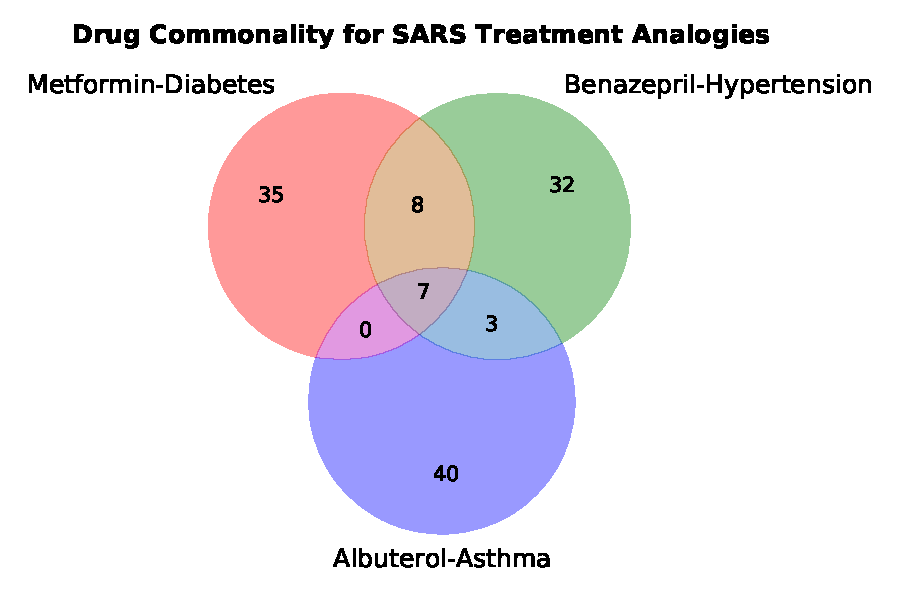
\includegraphics[width=0.7\textwidth]{drugvenn}
\caption{Venn diagram of the drug candidates identified by each SARS treatment analogy vector.}
\label{fig:drug_venn}
\end{figure}


% LIMITATIONS ---------------------------------------------
\section{Limitations}

Of course, while our method appears to have promise, it is not without limitations.
First, our method is limited to what has already been published in the scientific literature.
We also caution readers that these drugs have not been tested for COVID-19 efficacy, and we make no claims other than that some of these drugs deserve further exploration.
For example, we can say with some confidence that there are at least a few proposed drugs that are less promising.
Peramivir, and Tamiflu (oseltamivir), are neuraminidase inhibitors used to treat influenza.
While they are thus antivirals, coronaviruses do not use neuraminidase, so these particular drugs are less likely to be effective against SARS-CoV-2\cite{mccreary2020coronavirus}.
On the other hand, zanamivir, one of our marked positive controls\cite{hall2020search}, is also a neuraminidase inhibitor and should thus be a less likely candidate.
Nevertheless, we should expect to find false positives in our top hits along with true positives.
Finally, our embedding approach does not take into account the potential of drug-drug interactions to increase or decrease efficacy in any fashion.
All of this is to say that in vitro and in vivo experimentation, and observational EHR or claims data would all be useful sources of evidence for or against repurposing candidates listed here.


% CONCLUSION ----------------------------------------------
\section{Conclusion}

We present a word embedding mining approach to identifying candidate treatments for SARS-CoV-2 and COVID-19.
We first use a common drug-disease pair to produce a treatment analogy vector for SARS using a prebuilt biomedical word embedding.
We then use a simple word vector averaging approach to get word vectors for a list of FDA approved drugs and sort them by their distance to our treatment analogy vector.
Finally, we manually evaluate the top 50 candidate drugs and find several positive controls that have been suggested in the literature or are currently under investigation for SARS-CoV-2 or COVID-19 treatment.
While there are certain to be several false positives amongst our top hits as well, we find the presence of positive controls reassuring, and propose the remainder as potential candidates for further investigation.
We furthermore propose this word vector embedding approach in general as a useful tool for COVID-19 drug repurposing.
These results only scratch the surface of what is possible and we present this work as a suggestion to the community to investigate further.
Immediate avenues for future investigation include exploring more drug-disease analogy vectors, ranking drugs directly by their cosine similarity to proven treatments as they arise, and investigating drug-gene target analogy vectors rather than the disease treatment analogy we demonstrate here.

% REFERENCES ----------------------------------------------
\bibliographystyle{unsrt}
\bibliography{covid19_word_embed_mining}

\end{document}